\documentclass[10pt]{article}

\usepackage{hyperref}
\usepackage[margin=1in]{geometry} % landscape, 
\usepackage{pdflscape}
\usepackage{graphicx, float}
\usepackage{amsmath, amssymb}
\usepackage{longtable}

\title{SAR results for FCTC implementation Articles 5, 6, 8, 11, and 13}
\date{\today}

\usepackage{booktabs}

\begin{document}

\maketitle
\tableofcontents

This document presents the results from implementing an adjusted version of Aral et al. (2012)
propensity score matching estimator for evaluating contagion effects in the context of
the implementation of the FCTC.

Roughly, the method can be described as follows:

\begin{enumerate}
\item Define a treatment variable $Z_i$ which will be equal to 1 if an only
if individual $i$ is exposed to at least some percentage or number of neighbors
in the network that implemented at least one item of a particular article,
\item With $Z$ defined, via the MatchIt R package, we use the Coarsened
Exact Matching method (which maximizes balance). This returns a vector of weights $W$ that indicate whether
an individual $j$ was matched, hence $w_j>0$, or not, in which case $w_j=0$ and
compute an Average Treatment Effect on the Treated (ATT).
\item Finally, we estimated distributions for the ATT using bootstrapping
as described in Snijders and Borgatti (1999).
\end{enumerate}

\section{Posts network}

\begin{figure}[H]
	\centering
	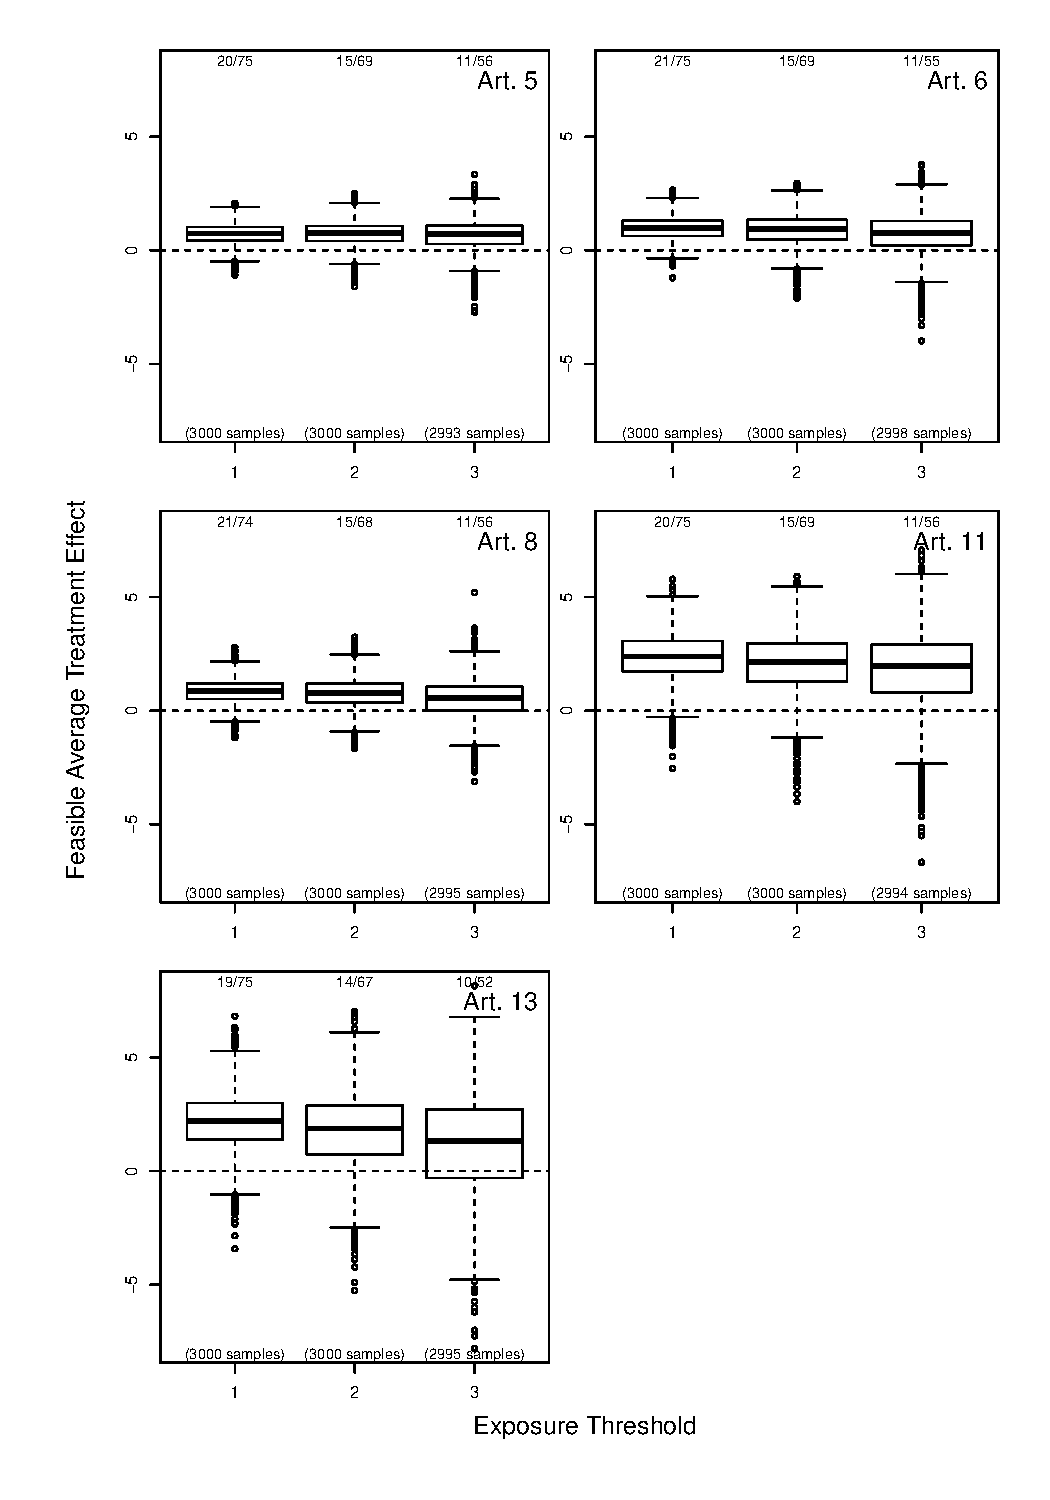
\includegraphics[width=.8\linewidth]{../fig/matching_bloxplot_adjmat_gl_posts.pdf}
	\caption{Distribution of Feasible Average Treatment Effect on the Treated using the GlobalLink posts network. Each box represents 2,000 bootstrap versions of the estimator.}
\end{figure}

\section{Robustness check}

In order to evaluate if the method reaches coherent results, we use it on a network
that, according to the SAR model, does show contagion effects, the centroid distance
network. Furthermore, we also performed the test on 2,000 permuted versions of this
network expecting to find no contagion effect.

\begin{figure}[H]
	\centering
	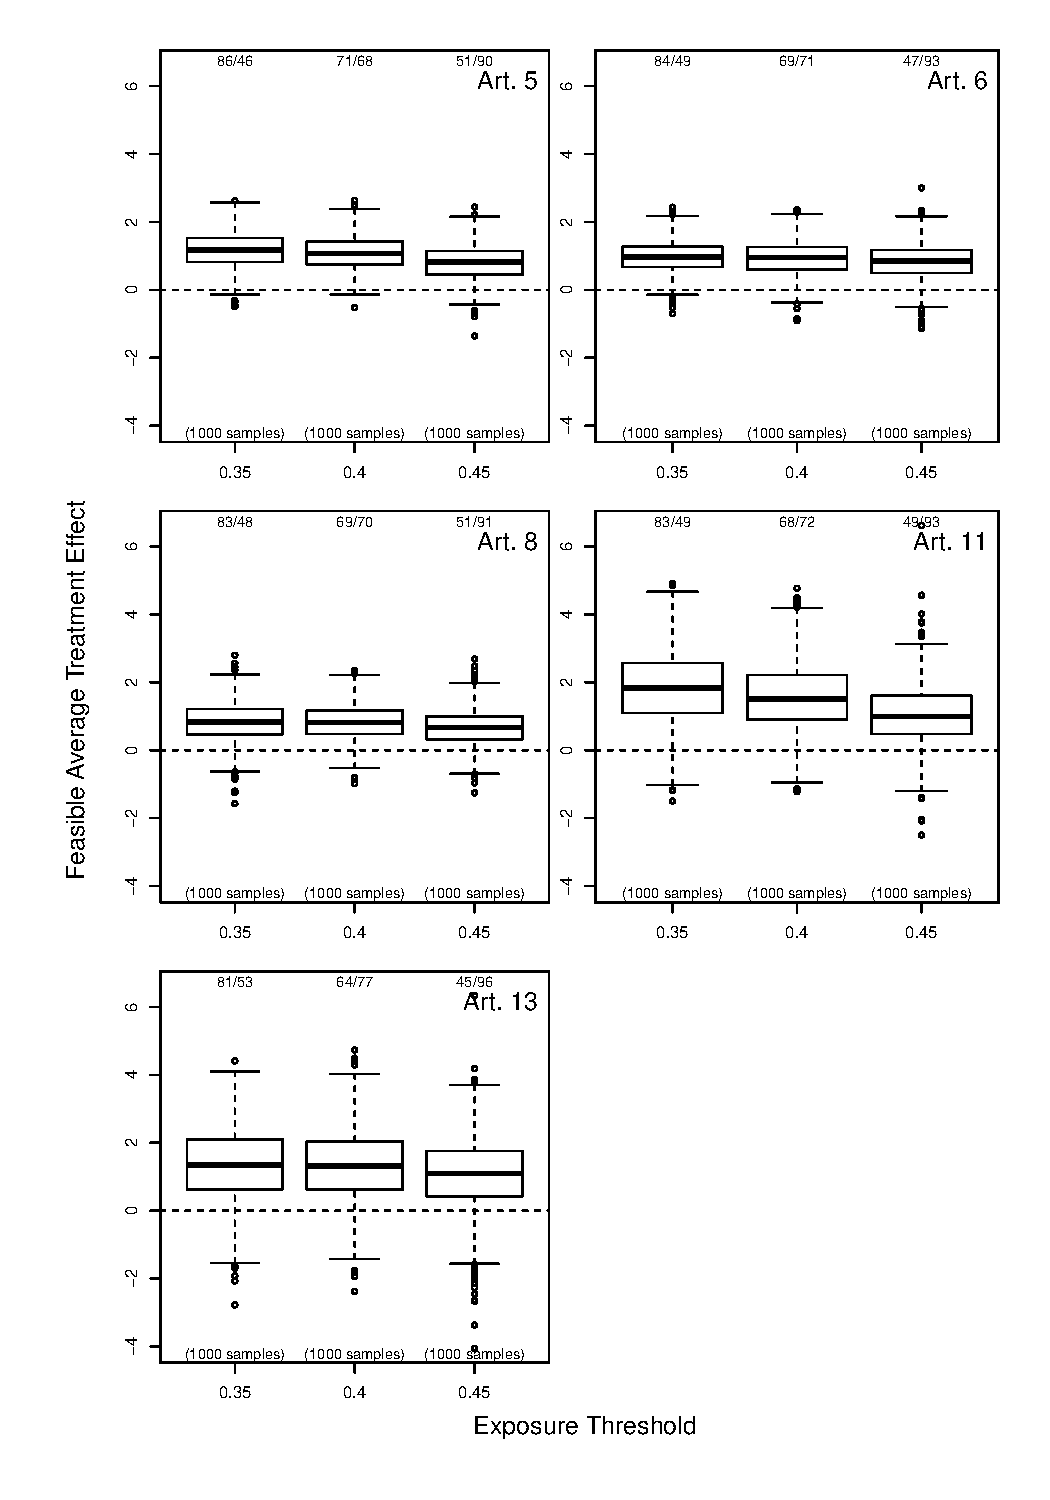
\includegraphics[width=.8\linewidth]{../fig/matching_bloxplot_adjmat_centroid_dist.pdf}
	\caption{Distribution of Sample Average Treatment Effect on the Treated using the Centroid Network. Each box represents 2,000 bootstrap versions of the estimator.}
\end{figure}

\begin{figure}[H]
	\centering
	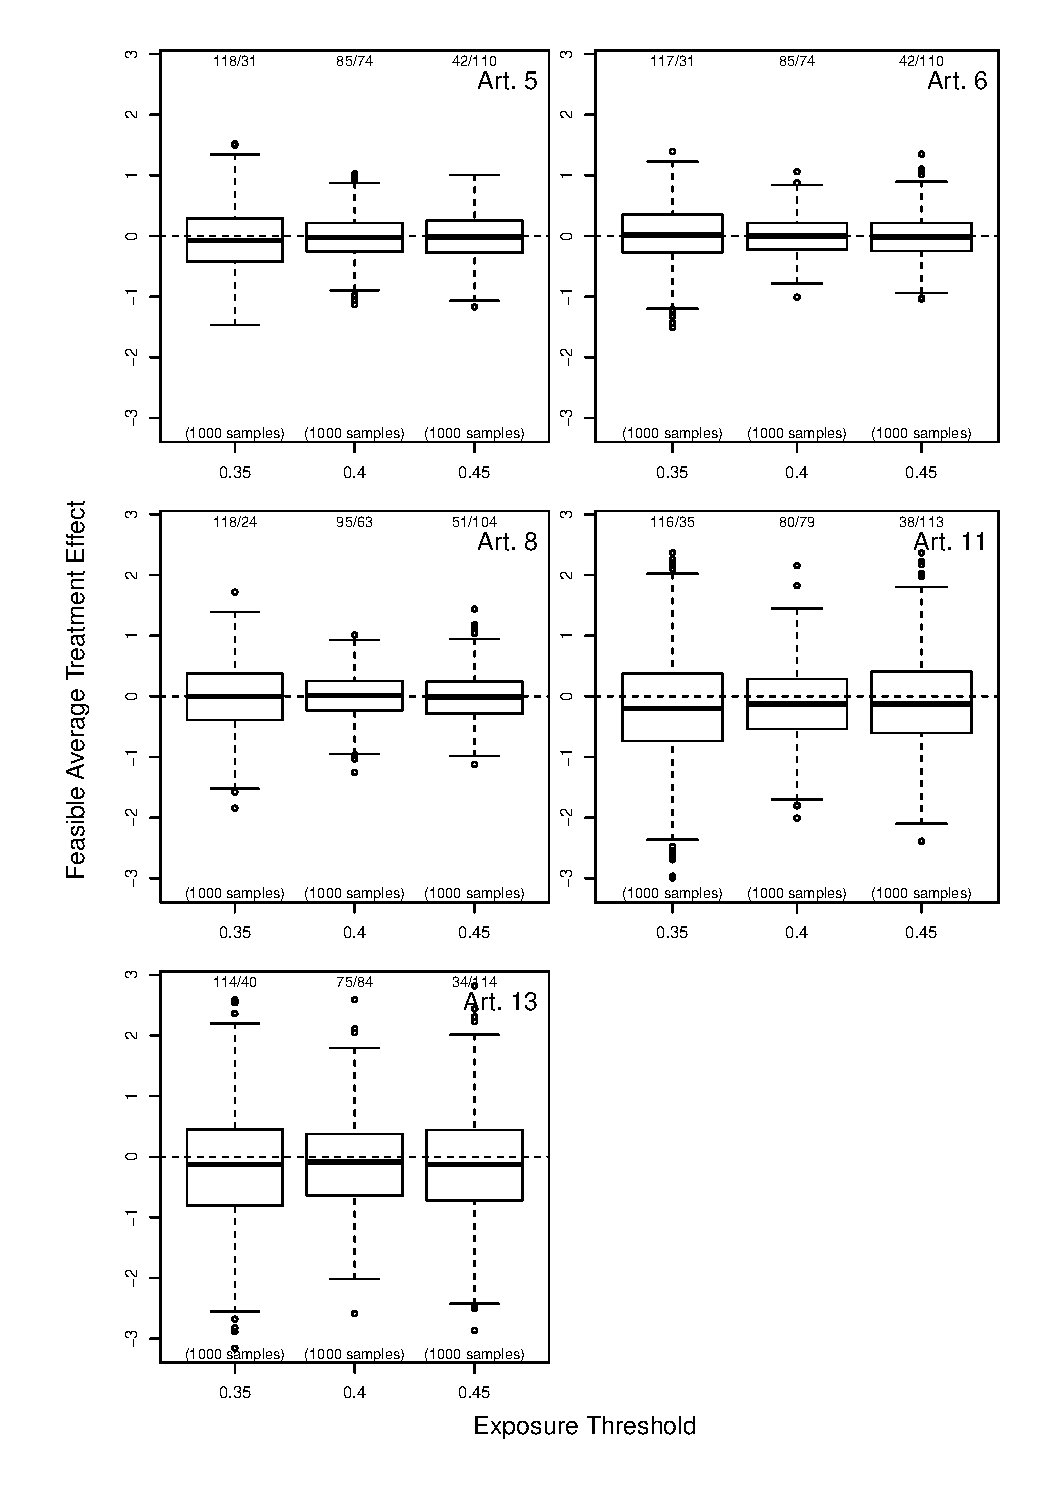
\includegraphics[width=.8\linewidth]{../fig/matching_bloxplot_dummy.pdf}
	\caption{Distribution of Feasible Average Treatment Effect on the Treated using a permuted version of the centroid network. Each box represents 2,000 bootstrap versions of the estimator.}
\end{figure}


% \begin{figure}[H]
% 	\centering
% 	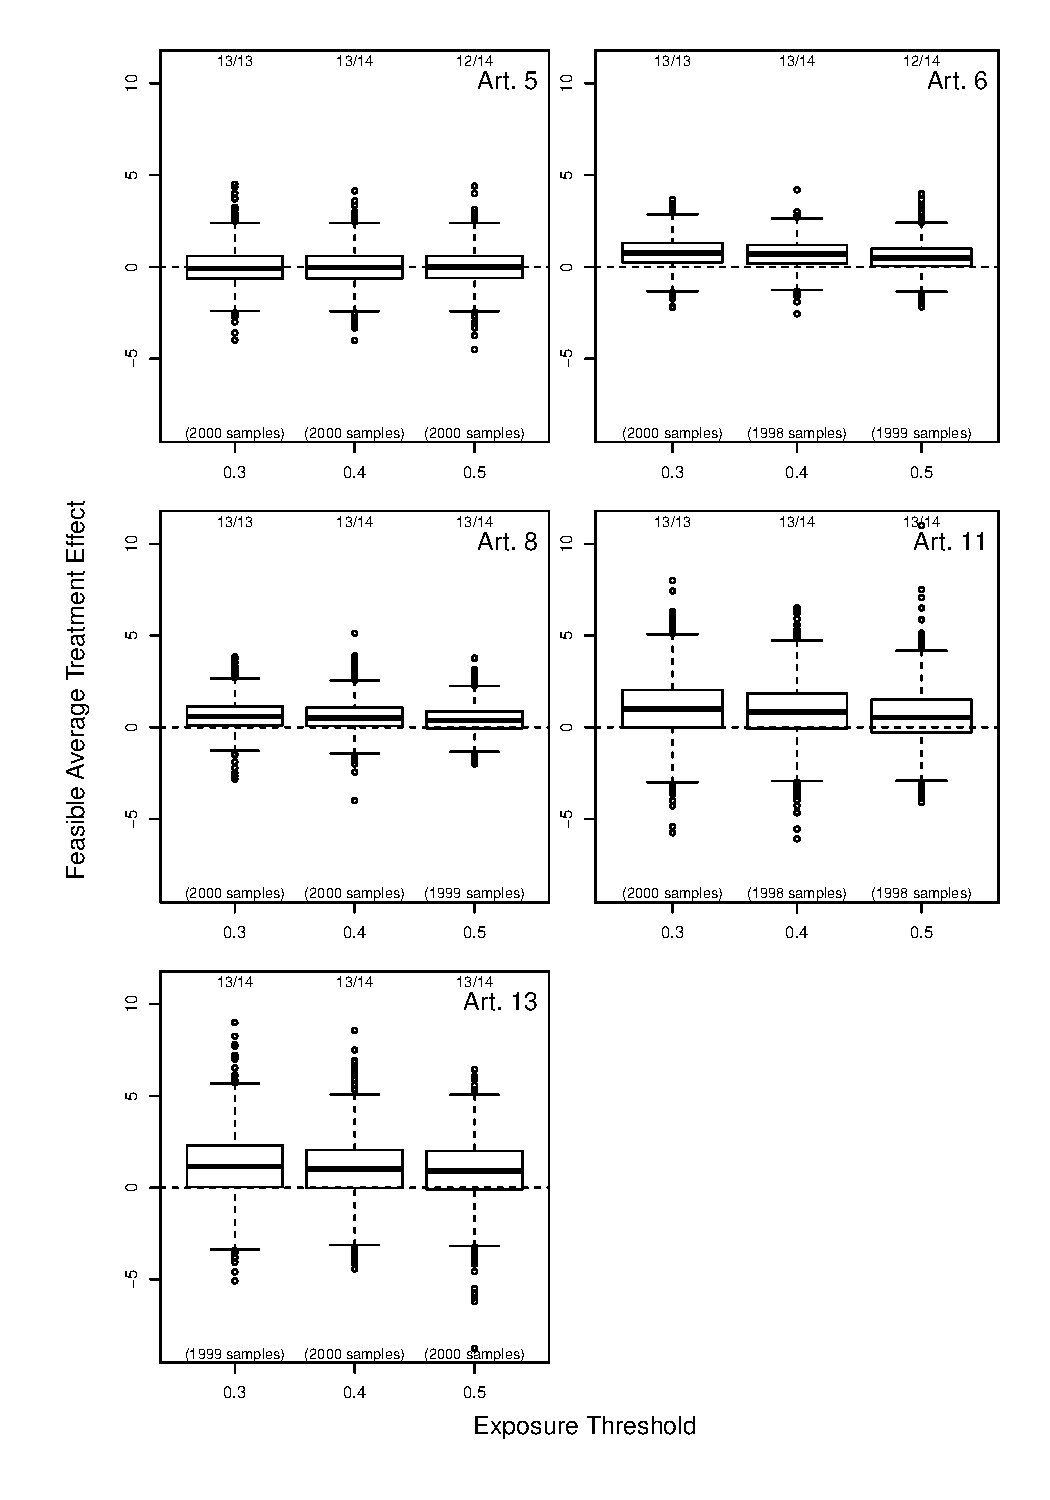
\includegraphics[width=.8\linewidth]{../fig/matching_bloxplot_adjmat_tobacco_trade.pdf}
% 	\caption{Distribution of Feasible Average Treatment Effect on the Treated using the FCTC COP Network. Each box represents 1,000 bootstrap versions of the estimator.}
% \end{figure}

\end{document}